\documentclass[fleqn, a4paper, 12pt, oneside]{amsart}
%\usepackage[top = 2cm, bottom = 1cm, left = 1cm, right = 1cm]{geometry}
\usepackage{exsheets, tasks}
\usepackage{amsmath, amssymb, amsthm} %standard AMS packages
\usepackage{marginnote} %marginnotes
\usepackage{gensymb} %miscellaneous symbols
\usepackage{commath} %differential symbols
\usepackage{xcolor} %colours
\usepackage{cancel} %cancelling terms
\usepackage{siunitx} %formatting units
\usepackage{tikz, pgfplots} %diagrams
\usetikzlibrary{calc, hobby, patterns, intersections}
\usepackage{graphicx} %inserting graphics
\usepackage{hyperref} %hyperlinks
\usepackage{datetime} %date and time
\usepackage{ulem} %underline for \emph{}
\usepackage{xfrac} %inline fractions
\usepackage{enumerate} %numbered lists
\usepackage{float} %inserting floats
\usepackage{circuitikz} %circuit diagrams

\newcommand\numberthis{\addtocounter{equation}{1}\tag{\theequation}} %adds numbers to specific equations in non-numbered list of equations

\newcommand{\AxisRotator}[1][rotate=0]{
	\tikz [x=0.25cm,y=0.60cm,line width=.2ex,-stealth,#1] \draw (0,0) arc (-150:150:1 and 1);%
} %rotation symbols on axes

\theoremstyle{definition}
\newtheorem{example}{Example}
\newtheorem{definition}{Definition}

\theoremstyle{theorem}
\newtheorem{theorem}{Theorem}

\newcommand{\curl}{\mathrm{curl\,}}

\makeatletter
\@addtoreset{section}{part} %resets section numbers in new part
\makeatother

\renewcommand{\thesubsection}{(\arabic{subsection})}
\renewcommand{\thesection}{(\arabic{section})}

%section headings on left
\makeatletter
\def\specialsection{\@startsection{section}{1}%
	\z@{\linespacing\@plus\linespacing}{.5\linespacing}%
	%  {\normalfont\centering}}% DELETED
	{\normalfont}}% NEW
\def\section{\@startsection{section}{1}%
	\z@{.7\linespacing\@plus\linespacing}{.5\linespacing}%
	%  {\normalfont\scshape\centering}}% DELETED
	{\normalfont\scshape}}% NEW
\makeatother

%forces newline after subsection
\makeatletter
\def\subsection{\@startsection{subsection}{3}%
	\z@{.5\linespacing\@plus.7\linespacing}{.1\linespacing}%
	{\normalfont\itshape}}
\makeatother

\settasks{counter-format = tsk[1].}

\SetupExSheets{solution/print = true}

%opening
\title{Physics 2 : Assignment 3}
\author
{
	Aakash Jog\\
	ID : 989323563
}
\date{\formatdate{15}{4}{2015}}

\begin{document}

\maketitle
%\setlength{\mathindent}{0pt}

\begin{question}
	Find the potential at distance $s$ from an infinitely long straight wire that carries a uniform line charge $\lambda$.
	Compute the gradient of your potential, and check that it yields the correct field.
\end{question}

\begin{solution}
	For an infinite line of charge, the charge at infinity is not zero.
	Therefore, it is wrong to assume that the electric potential at infinity is zero.
	\begin{align*}
		\varphi(s) - \varphi(r_0) &= -\int\limits_{r_0}^{s} \overrightarrow{E} \cdot \dif \overrightarrow{r}\\
		&= - \int\limits_{r_0}^{s} E \dif r\\
		&= - \int\limits_{r_0}^{s} \dfrac{\lambda}{2 \pi \varepsilon_0 r} \dif r\\
		&= \left. - \dfrac{\lambda}{2 \pi \varepsilon_0} \ln r \right|_{r_0}^{s}\\
		&= \dfrac{\lambda}{2 \pi \varepsilon_0} (\ln r_0 - \ln s)\\
		\therefore \varphi(s) &= \varphi(r_0) + \dfrac{\lambda}{2 \pi \varepsilon_0} (\ln r_0 - \ln s)
	\end{align*}
	If $\varphi(r_0)$, where $r_0 \neq 0$, $r_0 \neq \infty$, is set to be $0$, then,
	\begin{align*}
		\varphi(s) &= \dfrac{\lambda}{2 \pi \varepsilon_0} \left( \ln \dfrac{r_0}{s} \right)
	\end{align*}
	~\\
	\begin{align*}
		\nabla \varphi &= \nabla \left( \dfrac{\lambda}{2 \pi \varepsilon_0} \left( \ln \dfrac{r_0}{s} \right) \right)\\
		&= \dfrac{\lambda}{2 \pi \varepsilon_0} \dod{}{r} \left( \ln \dfrac{r_0}{s} \right)\\
		&= -\dfrac{\lambda}{2 \pi \varepsilon_0} \dod{}{r} \left( \ln \dfrac{s}{r_0} \right)\\
		\therefore -E &= -\dfrac{\lambda}{2 \pi \varepsilon_0} \dfrac{1}{s}\\
		\therefore E &= \dfrac{\lambda}{2 \pi \varepsilon_0} \dfrac{1}{s}
	\end{align*}
	This matches the known value of the electric field.
\end{solution}

\begin{question}
	A hollow spherical shell carries charge density $\rho = \dfrac{k}{r^2}$ in the region $a \le r \le b$.
	Find the potential at the centre, using infinity as your reference point.
	\begin{figure}[H]
		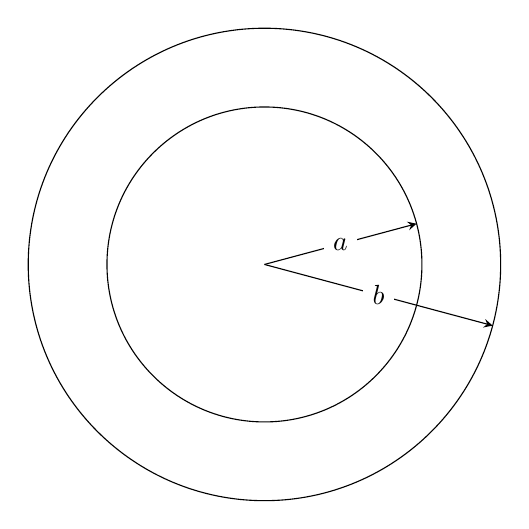
\begin{tikzpicture}
			\def\a{2};
			\def\b{3};
			\def\angle{15};
			
			\draw
				(0,0) circle (\a)
				(0,0) circle (\b);
			
			\begin{scope}[-stealth]
				\draw (0,0) -- (15:\a) node [midway, fill = white] {$a$};
				\draw (0,0) -- (-15:\b) node [midway, fill = white] {$b$};
			\end{scope}
		\end{tikzpicture}
	\end{figure}
\end{question}

\begin{solution}
	As $\varphi(\infty) = 0$, and as $E = \dod{\varphi}{r}$
	\begin{align*}
		\varphi(0) &= -\int\limits_{\infty}^{0} E \dif r\\
		&= \int\limits_{0}^{a} 0 \dif r + \int\limits_{a}^{b} \left( \dfrac{k}{\varepsilon_0} \dfrac{r - a}{r^2} \right) \dif r + \int\limits_{b}^{\infty} \left( \dfrac{k}{\varepsilon_0} \dfrac{b - a}{r^2} \right) \dif r\\
		&= 0 + \dfrac{k}{\varepsilon_0} \dfrac{b - a}{b} - \dfrac{k}{\varepsilon_0} \left( \ln \left( \dfrac{a}{b} \right) + 1 - \dfrac{a}{b} \right)\\
		&= \dfrac{k}{\varepsilon_0} \ln \dfrac{b}{a}
	\end{align*}
\end{solution}

\begin{question}
	A long coaxial cable carries a uniform volume charge density $\rho$ on the inner cylinder (radius $a$), and a uniform surface charge density on the outer cylindrical shell (radius b).
	This surface charge is negative and of just the right magnitude so that the cable as a whole is electrically neutral.
	Find the potential difference between a point on the axis and a point on the outer cylinder.
\end{question}

\begin{solution}
	\begin{align*}
		\varphi(b) - \varphi(0) &= -\int\limits_{0}^{b} E \dif r\\
		&= -\int\limits_{0}^{a} E \dif r - \int\limits_{a}^{b} E \dif r\\
		&= -\int\limits_{0}^{a} \dfrac{\rho r}{2 \varepsilon_0} \dif r - \int\limits_{a}^{b} \dfrac{\rho a^2}{2 \varepsilon_0 r} \dif r\\
		&= -\dfrac{\rho}{2 \varepsilon_0} \left( \dfrac{a^2}{2} \right) - \dfrac{\rho a^2}{2 \varepsilon_0} \left( \ln b - \ln a \right)\\
		&= -\dfrac{\rho a^2}{4 \varepsilon_0} \left( 1 + 2 \ln \dfrac{b}{a} \right)
	\end{align*}
\end{solution}

\begin{question}
	A conical surface (an empty ice-cream cone) carries a uniform surface charge $\sigma$.
	The height of the cone is $h$, as is the radius of the top.
	Find the potential difference between points $\mathrm{a}$ (the vertex) and $\mathrm{b}$ (the centre of the top).
\end{question}

\begin{solution}
	\begin{figure}[H]
		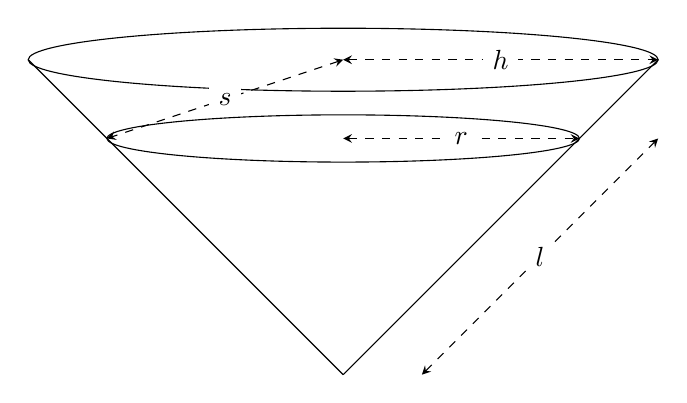
\begin{tikzpicture}
			\def\H{4};
			\def\R{4};
			\def\h{3};
			\def\r{3};
			
			\coordinate (apex) at (0,0);
			\coordinate (base centre) at (0,\H);
			\coordinate (elemental ring centre) at (0,\h);
			
			\draw (base centre) circle [x radius = \R, y radius = 0.1*\R];
			\draw ($ (base centre) + (-\H,0) $) -- (apex);
			\draw ($ (base centre) + (\H,0) $) -- (apex);
			
			\draw (elemental ring centre) circle [x radius = \r, y radius = 0.1*\r];
			
			\begin{scope}[dashed, stealth-stealth]
				\draw (base centre) -- ++(\R,0) node [midway, fill = white] {$h$};
				\draw (elemental ring centre) -- ++(\r,0) node [midway, fill = white] {$r$};
				\draw ($ (apex) + (1,0) $) -- ($ (elemental ring centre) + (\r,0) + (1,0) $) node [midway, fill = white] {$l$};
				\draw (base centre) -- ($ (elemental ring centre) + (-\r,0) $) node [midway, fill = white] {$s$};
			\end{scope}
		\end{tikzpicture}
	\end{figure}
	Consider an elemental ring of radius $r$ and thickness $\dif r$ as shown.\\
	Let $s$ be the distance from the centre of the base to any point on the elemental ring.\\
	Therefore,
	\begin{align*}
		\varphi(a) &= \int \dfrac{k \dif q}{l}\\
		&= \int\limits_{0}^{\sqrt{2} h} \dfrac{k \sigma \cdot 2 \pi r}{l} \dif l\\
		&= \int\limits_{0}^{\sqrt{2} h} \dfrac{2 k \sigma \pi r}{\sqrt{2} r} \dif l\\
		&= \dfrac{2 k \sigma \pi}{\sqrt{2}} \cdot \sqrt{2} h\\
		&= \dfrac{\sigma h}{2 \varepsilon_0}
	\end{align*}
	\begin{align*}
		\varphi(b) &= \int \dfrac{k \dif q}{s}\\
		&= \int\limits_{0}^{\sqrt{2} h} \dfrac{k \sigma \cdot 2 \pi r}{\sqrt{h^2 + l^2 - \sqrt{2} h l}} \dif l\\
		&= \left. \dfrac{2 k \sigma \pi}{\sqrt{2}} \left( \sqrt{h^2 + l^2 - \sqrt{2} h l} \right) \right|_{0}^{\sqrt{2}}\\
		&\quad + \left. \dfrac{2 k \sigma \pi}{\sqrt{2}} \left( \dfrac{h}{\sqrt{2}} \ln \left( 2 \sqrt{h^2 + l^2 - \sqrt{2} h l} + 2 l - \sqrt{2} h \right) \right) \right|_{0}^{\sqrt{2}} \\
		&= \dfrac{\sigma h}{4 \varepsilon_0} \ln \left( 3 + 2 \sqrt{2} \right)\\
		&= \dfrac{\sigma h}{2 \varepsilon_0} \ln \left( 1 + \sqrt{2} \right)
	\end{align*}
	Therefore,
	\begin{align*}
		\varphi(a) - \varphi(b) &= \dfrac{\sigma h}{2 \varepsilon_0} \left( 1 - \ln \left( 1 + \sqrt{2} \right) \right)
	\end{align*}
\end{solution}

\begin{question}
	Find the potential at a distance $z$ above the centre of the charge distributions shown.
	In each case, compute $\overrightarrow{E} = \overrightarrow{\nabla} \varphi$, and compare your answers with the fields computed last week.
	Suppose that we changed the right-hand charge in the first figure to $-q$; what then is the potential at $\mathrm{P}$?
	What field does that suggest?
	Explain.
	\begin{enumerate}
		\item
			\begin{figure}[H]
				\begin{tikzpicture}
					\def\z{3};
					\def\d{4};
					
					\coordinate (q1) at ({-\d/2},0);
					\coordinate (q2) at ({\d/2},0);
					\coordinate (P) at (0,\z);
					
					\begin{scope}
						\filldraw (q1) circle (2pt) node [below] {$q$};
						\filldraw (q2) circle (2pt) node [below] {$q$};
						
						\node [below] at (0,0) {$d$};
						\node [left] at (0,\z/2) {$z$};
						
						\filldraw (P) circle (1pt) node [right] {$\mathrm{P}$};
					\end{scope}
					
					\begin{scope}
						\draw ($ (q1) + (-1,0) $) -- ($ (q2) + (1,0) $);
						\draw ($ (P) + (0,1) $) -- (0,0);
					\end{scope}
				\end{tikzpicture}
			\end{figure}
		\item
			\begin{figure}[H]
				\begin{tikzpicture}
					\def\z{3};
					\def\L{2};
					
					\coordinate (q1) at ({-\L},0);
					\coordinate (q2) at ({\L},0);
					\coordinate (P) at (0,\z);
					
					\begin{scope}
						\draw [ultra thick] (q1) -- (q2) node [midway, below] {$2L$} node [midway, above left] {$\lambda$};
						
						\node [left] at (0,\z/2) {$z$};
						
						\filldraw (P) circle (1pt) node [right] {$\mathrm{P}$};
					\end{scope}
					
					\begin{scope}
						\draw ($ (q1) + (-1,0) $) -- ($ (q2) + (1,0) $);
						\draw ($ (P) + (0,1) $) -- (0,0);
					\end{scope}
				\end{tikzpicture}
			\end{figure}
		\item
			\begin{figure}[H]
				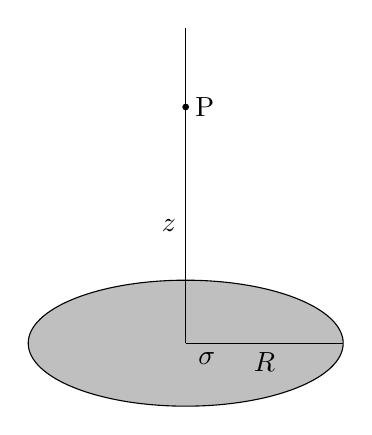
\begin{tikzpicture}
					\def\z{3};
					\def\R{2};
					
					\coordinate (q1) at ({-\R},0);
					\coordinate (q2) at ({\R},0);
					\coordinate (P) at (0,\z);
					
					\begin{scope}
						\draw [fill = lightgray] (0,0) circle [x radius = \R, y radius = 0.4*\R];
						
						\node [left] at (0,\z/2) {$z$};
						
						\filldraw (P) circle (1pt) node [right] {$\mathrm{P}$};
					\end{scope}
					
					\begin{scope}
						\draw (0,0) -- (\R,0) node [midway, below] {$R$} node [near start, below left] {$\sigma$};
						\draw ($ (P) + (0,1) $) -- (0,0);
					\end{scope}
				\end{tikzpicture}
			\end{figure}
	\end{enumerate}
\end{question}

\begin{solution}
	\begin{enumerate}
		\item
			\begin{align*}
				\varphi &= 2 \cdot \dfrac{1}{4 \pi \varepsilon_0} \dfrac{q}{\sqrt{\sfrac{d^2}{4} + z^2}}
			\end{align*}
			~\\
			By symmetry,
			\begin{equation*}
				E_x = E_y = 0
			\end{equation*}
			Therefore,
			\begin{align*}
				E_z &= -\dod{}{z} \varphi\\
				&= -\dod{}{z} \left( \dfrac{1}{4 \pi \varepsilon_0} \dfrac{2q}{\sqrt{\sfrac{d^2}{4} + z^2}} \right)\\
				&= \dfrac{1}{4 \pi \varepsilon_0} \dfrac{2q}{\left( \sfrac{d^2}{4} + z^2 \right)^{\sfrac{3}{2}}}
			\end{align*}
			This is consistent with the known electric field.\\
			~\\
			If the right-hand charge is changed to $-q$,
			\begin{align*}
				\varphi &= \dfrac{1}{4 \pi \varepsilon}{q}{\sqrt{\sfrac{d^2}{4} + z^2}} + \dfrac{1}{4 \pi \varepsilon}{-q}{\sqrt{\sfrac{d^2}{4} + z^2}}\\
				&= 0
			\end{align*}\\
			Therefore, $E_z = 0$, therefore, the field must be in the horizontal direction only.
		\item
			\begin{align*}
				\varphi &= \int\limits_{-L}^{L} \dfrac{1}{4 \pi \varepsilon_0} \dfrac{\lambda \dif x}{\sqrt{x^2 + z^2}}\\
				&= \dfrac{\lambda}{4 \pi \varepsilon_0} \left. \ln \left( x + \sqrt{x^2 + z^2} \right) \right|_{-L}{L}\\
				&= \dfrac{\lambda}{2 \pi \varepsilon_0} \ln \left( \dfrac{L + \sqrt{L^2 + z^2}}{z} \right)
			\end{align*}
			~\\
			By symmetry,
			\begin{equation*}
				E_x = E_y = 0
			\end{equation*}
			Therefore,
			\begin{align*}
				E_z &= -\dod{}{z} \varphi\\
				&= -\dod{}{z} \left( \dfrac{\lambda}{2 \pi \varepsilon_0} \ln \left( \dfrac{L + \sqrt{L^2 + z^2}}{z} \right) \right)\\
				&= \dfrac{\lambda}{2 \pi \varepsilon_0} \dfrac{L}{z \sqrt{z^2 + L^2}}
			\end{align*}
			This is consistent with the known electric field.
		\item
			Considering the ring to be made up of elemental rings,
			\begin{align*}
				\varphi &= \int\limits_{0}^{R} \dfrac{1}{4 \pi \varepsilon_0} \dfrac{\sigma \cdot 2 \pi r \dif r}{\sqrt{r^2 + z^2}}\\
				&= \dfrac{\sigma}{2 \varepsilon_0} \int\limits_{0}^{R} \dfrac{r}{\sqrt{r^2 + z^2}} \dif r\\
				&= \dfrac{\sigma}{2 \varepsilon_0} \left. \sqrt{r^2 + z^2} \right|_{0}^{R}\\
				&= \dfrac{\sigma}{2 \varepsilon_0} \left( \sqrt{R^2 + z^2} - z \right)
			\end{align*}
			By symmetry,
			\begin{equation*}
				E_x = E_y = 0
			\end{equation*}
			Therefore,
			\begin{align*}
				E_z &= -\dod{}{z} \varphi\\
				&= -\dod{}{z} \left( \dfrac{\sigma}{2 \varepsilon_0} \left( \sqrt{R^2 + z^2} - z \right) \right)\\
				&= \dfrac{\sigma}{2 \varepsilon_0} \left( 1 - \dfrac{z}{\sqrt{R^2 + z^2}} \right)
			\end{align*}
			This is consistent with the known electric field.
	\end{enumerate}
\end{solution}

\end{document}
